\documentclass[11pt,a4paper]{article}
\usepackage{graphicx}
\usepackage{amsmath,amssymb,amsthm,amsfonts}
\usepackage{geometry}\geometry{left=2.3cm,right=2.3cm,top=2.5cm,bottom=2.5cm}
\usepackage{setspace}\setstretch{1.20}
\usepackage{hyperref}\hypersetup{colorlinks=true,linkcolor=black,citecolor=black}
\usepackage{parskip,booktabs,array,xcolor,titlesec,enumitem}
\titleformat{\section}{\large\bfseries}{}{0em}{}[\titlerule]
\titlespacing{\section}{0pt}{14pt}{6pt}
\titleformat{\subsection}{\normalsize\bfseries}{\thesubsection\;}{0em}{}
\newtheorem{remark}{Remark}
\begin{document}
\begin{center}
{\LARGE\bfseries Numerical Protocol}\\[0.3cm]
{\large Zumbach Effect: ESN vs.\ the PDV-GL Model Used as Ground-Truth DGP}\\[0.2cm]
{\normalsize Othmane Zarhali}
\end{center}
\vspace{0.15cm}\noindent\rule{\textwidth}{0.8pt}

\begin{abstract}

The Zumbach-effect time-reversal asymmetry effect experiment is conducted according to the following
steps:

\begin{enumerate}
    \item \textbf{Data generation.} Use the \textbf{4-factor Markovian}
    Guyon \& Lekeufack path-dependent volatility model (PDV-GL)
    \cite{guyon2023} as the ground-truth data-generating process (DGP).
    The simulation employs the literature-calibrated
    ``Table~8, Parameter Set~1 (Realistic paths)'' parameters,
    \[
    \beta_0=0.04,\;
    \beta_1=-0.13,\;
    \beta_2=0.65,\;
    \beta_{1,2}=0,
    \]
    \[
    \lambda_{1,0}=55,\;
    \lambda_{1,1}=10,\;
    \theta_1=0.25,\;
    \lambda_{2,0}=20,\;
    \lambda_{2,1}=3,\;
    \theta_2=0.5,
    \]
    which are subsequently rescaled to a common annualised volatility
    target of $20\%$ (Section~1). This defines a single, fully specified
    benchmark scenario without parameter sweeps.

    \item \textbf{Model calibration.} Calibrate only the ESN A2-981003
    and Quadratic Rough Heston (QRH) models to the stylised-fact profile
    of the PDV-GL DGP. A separately calibrated copy of PDV-GL is
    intentionally omitted, since the DGP itself already represents the
    reference model.

    Both models are calibrated using the complete 11-term
    data-adaptive score $S$ (Eq.~\eqref{eq:score}), together with the
    smooth Gaussian-kernel proximity function.

    \item \textbf{ESN parameterisation.} The ESN is evaluated using its
    current optimal architecture,
    \[
    (N_r,N_z)=(96,12),
    \]
    with a read-out composed of
    \begin{itemize}
        \item a linear roughness factor;
        \item a per-mode $z$-readout profile;
        \item a symmetric quadratic reservoir-state interaction matrix.
    \end{itemize}
    These components are jointly calibrated with the Hurst exponent and
    the reservoir rate bounds (Section~\ref{sec:calib}).

    \item \textbf{Model evaluation.} Assess the ability of the calibrated
    models to reproduce the Zumbach time-reversal asymmetry of the DGP
    using
    \begin{itemize}
        \item the lag-dependent Zumbach curve $Z(L)$;
        \item the aggregate statistic
        \[
        Z=\frac{1}{3}\left[Z(5)+Z(10)+Z(20)\right];
        \]
        \item complementary diagnostics, including the leverage
        autocorrelation function, volatility autocorrelation function,
        and return-tail statistics.
    \end{itemize}
\end{enumerate}
\end{abstract}

\tableofcontents\vspace{0.4cm}

\section{DGP: PDV-GL as Ground Truth}

The data-generating process is the Guyon \& Lekeufack path-dependent
volatility model \cite{guyon2023}, in its \textbf{4-factor Markovian}
form -- the standard finite-dimensional approximation obtained by
replacing each power-law memory kernel with a mixture of two
exponential (OU-type) kernels, making the model fast to simulate as a
genuine Markov process:
\begin{equation}
  \frac{dS_t}{S_t} = \sigma_t\,dW_t,
  \label{eq:pdvgl_ret}
\end{equation}
\begin{equation}
  \sigma_t = \beta_0 + \beta_1 R_{1,t} + \beta_2\sqrt{R_{2,t}} + \beta_{1,2}\,R_{1,t}\sqrt{R_{2,t}},
  \label{eq:pdvgl_var}
\end{equation}
\begin{equation}
  R_{1,t} = \theta_1 X_{1,0,t} + (1-\theta_1) X_{1,1,t},
  \qquad
  R_{2,t} = \theta_2 X_{2,0,t} + (1-\theta_2) X_{2,1,t},
  \label{eq:pdvgl_factors}
\end{equation}
where $X_{1,j,t}$ is an exponentially-weighted moving average of past
\emph{signed} returns with mean-reversion rate $\lambda_{1,j}$ (the
\textbf{leverage} factor, a mixture of a fast and a slow exponential
kernel), and $X_{2,j,t}$ is an EWMA of past \emph{squared} returns with
rate $\lambda_{2,j}$ (the \textbf{magnitude} factor). Unlike every
other DGP in this line of protocols, PDV-GL is used here as
\textbf{ground truth}, not as a candidate model.

\paragraph{"True" parameters -- literature-calibrated Table 8,
Parameter Set 1 (Realistic paths).}
\begin{table}[H]
\centering
\caption{PDV-GL 4-factor Markovian ground-truth parameters (Table 8, Parameter Set 1).}
\label{tab:pdvgl4f}
\begin{tabular}{@{}lr@{}}
\toprule
Parameter & Value \\
\midrule
$\beta_0$ & 0.04 \\
$\beta_1$ & $-0.13$ \\
$\beta_2$ & 0.65 \\
$\beta_{1,2}$ & 0 (unused for Set 1) \\
$\lambda_{1,0}$ & 55 \\
$\lambda_{1,1}$ & 10 \\
$\theta_1$ & 0.25 \\
$\lambda_{2,0}$ & 20 \\
$\lambda_{2,1}$ & 3 \\
$\theta_2$ & 0.5 \\
\bottomrule
\end{tabular}
\end{table}
$\lambda$ rates are in annualised units; each is applied at the daily
step via $e^{-\lambda\Delta t}$, $\Delta t=1/252$.

\paragraph{Rescaling.}
Run literally with these parameters (and daily returns in decimal
units), the model's realised annualised volatility comes out at only
$\approx4\%$ -- the source table's implicit return-scale convention
could not be verified from the parameters alone. A single, documented
linear rescaling $X\mapsto X\cdot(\mathrm{TV\_DAY}/\widehat\sigma)$ is
applied post-hoc to bring the level to the same $20\%$ annualised target
used throughout this line of protocols. This is a pure amplitude change:
every \emph{normalised} statistic used in this protocol ($\hat H$,
kurtosis, leverage correlation, and the $Z(\tau)/\sigma^3$ cross-moment
ratio) is left \textbf{exactly unchanged}, since numerator and
denominator scale identically under a uniform linear rescaling.

\paragraph{Zumbach effect mechanism.}
Because $\beta_1<0$, a large \emph{negative} past return raises
$R_{1,t}$ with the sign needed to raise $\sigma_t$ and hence future
variance -- a genuine, signed leverage asymmetry. At these literature
parameters, the realised leverage correlation is $\approx-0.04$ to
$-0.17$ depending on the exact path sample, and the windowed Zumbach
scalar $Z$ (Eq.~\ref{eq:score}'s calibration statistic) comes out
strongly positive ($Z\approx0.22$ in the run reported here) -- a
clearly non-trivial, sustained effect rather than a borderline one.

\paragraph{Simulation.}
Eq.~\eqref{eq:pdvgl_factors} is iterated as an exact discretisation of
the four OU-type factors ($X_{1,0},X_{1,1},X_{2,0},X_{2,1}$) at the
daily step, using $e^{-\lambda_{i,j}\Delta t}$ decay -- a genuine Markov
process in $(X_{1,0},X_{1,1},X_{2,0},X_{2,1})$, no path history storage
needed (unlike the power-law-kernel DGPs used elsewhere in this line of
protocols).

\paragraph{Parameter grid.}
None -- Parameter Set 1 is a single, fully-specified literature
calibration (Table~\ref{tab:pdvgl4f}); every path uses the same fixed
parameters.

\section{Models}
\subsection{ESN A2-981003 (current optimal architecture)}

The ESN uses Gaussian Brownian innovations, with 7 shared
hyperparameters and $N_r=96,N_z=12$. \texttt{rough\_scale} and the
$z$-readout ($\texttt{zr\_lo},\texttt{zr\_hi}$, plus the symmetric
quadratic matrix coefficients $(m_1,m_2)$) are calibrated per DGP cell
(\S\ref{sec:calib}), not part of this fixed table.
\begin{table}[H]
\centering
\caption{The 7 shared hyperparameters of the optimal architecture.}
\label{tab:optarch}
\begin{tabular}{@{}lr@{}}
\toprule
Hyperparameter & Value \\
\midrule
$N_r$ & 96 \\
$N_z$ & 12 \\
\texttt{z\_strength} & 0.1929 \\
\texttt{even\_strength} & 2.2291 \\
\texttt{linear\_strength} & 0.1930 \\
\texttt{gamma\_norm} & 0.9651 \\
\texttt{local\_z\_strength} & 0.0476 \\
\texttt{zz\_scale} & 0.0397 \\
\texttt{sign\_prob\_neg} & 0.2219 \\
\texttt{rough\_orientation} & $-1.0$ (fixed) \\

\end{tabular}
\end{table}
Single $\varepsilon_t\sim\mathcal{N}(0,1)$ drives both the Ito log-return
and the diagonal OU rough bank. The negative instantaneous leverage
$\kappa_0=-0.434991<0$ (admissibility, guaranteed by construction) gives
the ESN an endogenous Zumbach-like asymmetry -- structurally different
from PDV-GL's own path-dependent-feedback mechanism (\S1), so a good
match here is evidence the ESN's mechanism can \emph{mimic} the effect,
not that it replicates the same causal channel. $H$, the $r$-layer rate
window $[\lambda_{\rm lo},\lambda_{\rm hi}]$, and the $z$-layer rate
window $[a_{\rm lo},a_{\rm hi}]$ are \textbf{calibrated per $\alpha_r$
DGP cell} (\S\ref{sec:calib}) -- they are not part of the shared
architecture above.

\subsection{Quadratic Rough Heston (QRH)}
Bourgey \& Gatheral: $V_t=Y_t^2+c$, gamma kernel
$\kappa(\tau)=\nu/\Gamma(\alpha)\tau^{\alpha-1}e^{-\lambda\tau}$,
$\alpha=H+\tfrac{1}{2}$, Euler-Volterra with 252-step ring buffer.
Included alongside the ESN as a second, structurally different
candidate model (a genuine rough-volatility SDE, vs.\ the ESN's
Markovian reservoir approximation) against the same PDV-GL ground truth.

\section{Calibration: Full 11-Term Score, Smooth Kernel}
\label{sec:calib}

The data-adaptive score (identical structure to every other protocol in
this series, Eq.~\eqref{eq:score}), with the \textbf{smooth
Gaussian-kernel} proximity (protocol V5) rather than the original
piecewise-linear tent:
\begin{equation}
\begin{aligned}
S &= 2.2\,\bigl(1-f(\hat H)\bigr)+1.4\,\bigl(1-f(\bar\sigma)\bigr)+0.6\,\bigl(1-g(q_{995})\bigr)+0.2\,\bigl(1-g(\sigma_{\max})\bigr)\\
  &+0.8\,\bigl(1-f(\bar V_{\mathrm{ACF}})\bigr)+1.0\,\bigl(1-f(G_T)\bigr)+0.8\,\bigl(1-f(F_T)\bigr)+\mathbf{3.5}\,\bigl(1-f(Z)\bigr)\\
  &+1.1\,\bigl(1-f(L)\bigr)+0.7\,\bigl(1-f(K)\bigr)+0.5\,\bigl(1-f(A)\bigr)+5\cdot\mathrm{Stress},
\end{aligned}
\label{eq:score}
\end{equation}
where $f(x,c,s)=\exp(-\tfrac12((x-c)/s)^2)$,
$g(x,c,s)=\exp(-\tfrac12((x-c)_+/s)^2)$, both in $(0,1]$. $S\geq0$ is
\textbf{minimised directly} (no sign flip); $S=0$ is a perfect match on
all 11 stylised facts and no stress event; \textbf{$S=17.8$ is
worst-possible} (raised from $15.3$ by the Zumbach-weight increase
below). All centres $c_k$ and tolerances $s_k$ are DGP cross-path mean
and $\max(\mathrm{std},0.30|c_k|,\mathrm{floor}_k)$.

\paragraph{Zumbach score weighting.} The Zumbach weight is raised
from $1.0$ to $\mathbf{3.5}$ -- now the single largest weight in $S$,
exceeding even $\hat H$'s $2.2$ -- and QRH's calibration uses a
2-point multi-start. \S\ref{sec:zumbach-results} reports the full
root-cause diagnosis and result.

\paragraph{ESN read-out.} The ESN's read-out combines a linear rough
factor, a per-mode $z$-readout profile
$(\texttt{zr\_lo},\texttt{zr\_hi})$, and a symmetric quadratic-term
matrix $Q=(1/N_r)(m_1I+m_2qq^\top)$ added to the pre-activation. The
ESN calibrates its full inner-loop vector
\[
H,\ \lambda_{\rm lo},\ \lambda_{\rm hi},\ a_{\rm lo},\ a_{\rm hi},\
\Delta b_0,\ \mathrm{scale},\ \texttt{rough\_scale},\
\texttt{zr\_lo},\ \texttt{zr\_hi},\ m_1,\ m_2
\]
-- \textbf{12 dimensions} -- via an 11-point multi-start
Nelder--Mead scheme (rough/fast, persistent/slow, intermediate,
wide-band/multiscale, long-memory extreme, Zumbach
term1/term2-balanced, strong-amplitude, weak-amplitude,
isotropic-positive, isotropic-negative, and $q$-aligned-positive
starts), keeping the best-of-eleven result; only the 7 shared
architecture hyperparameters of Table~\ref{tab:optarch} stay fixed.

Calibrated parameters:
\begin{center}\renewcommand{\arraystretch}{1.3}
\begin{tabular}{@{}p{3.0cm}p{6.4cm}p{5.0cm}@{}}\toprule
Model & Parameters calibrated & Remark \\\midrule
ESN A2-981003 & $H$, $\lambda_{\rm lo}$, $\lambda_{\rm hi}$, $a_{\rm lo}$,
  $a_{\rm hi}$, $\Delta b_0$, scale $s$, \texttt{rough\_scale},
  \texttt{zr\_lo}, \texttt{zr\_hi}, $m_1$, $m_2$ &
  7 shared hyperparameters fixed; full 12-dim.\ inner-loop calibrated
  per $\alpha_r$ cell (11-start Nelder--Mead) \\
QRH & $H,\nu_{\rm vol},\lambda,c_{\rm frac}$ & 2-start Nelder--Mead
  (added a low-$H$ start; see \S\ref{sec:zumbach-results}) \\
\bottomrule\end{tabular}\end{center}


\section{Zumbach Diagnostic}
\label{sec:windowed}

\begin{equation}
  Z(L) = \mathrm{Corr}\!\bigl(\mathrm{past}_L R^2,\,\mathrm{fut}_L V\bigr)
        - \mathrm{Corr}\!\bigl(\mathrm{past}_L V,\,\mathrm{fut}_L R^2\bigr),
  \label{eq:zumbach_scalar}
\end{equation}
where $\mathrm{past}_L R^2=(X_t{-}X_{t-L})^2$ and
$\mathrm{fut}_L V=(V_{t+L}{-}V_t)/L$. $Z(L)>0$ means the
past-magnitude$\to$future-vol channel [$\mathrm{Corr}(\mathrm{past}_LR^2,\mathrm{fut}_LV)$]
dominates the reverse, time-reversed channel
[$\mathrm{Corr}(\mathrm{past}_LV,\mathrm{fut}_LR^2)$] -- the genuine
Zumbach / time-reversal-asymmetry signature. This is the SAME windowed,
correlation-based metric used for calibration (the scalar
$Z=\tfrac{1}{3}[Z(5){+}Z(10){+}Z(20)]$ enters the score with weight
1.0) and for Figure Z1. It depends only on magnitudes, not the sign of
returns, and so is well-defined even for DGPs with no leverage term at
all.

The ESN carries its own, structurally distinct source of asymmetry (the
fixed $\kappa_0<0$ leverage built into its architecture, \S2) and the
PDV-GL DGP its own path-dependent feedback (\S1) -- a good match
between the ESN's and the DGP's $Z(L)$ is therefore evidence that the
ESN's mechanism can \emph{mimic} the magnitude of the effect, not that
it reproduces the same causal channel.

\begin{figure}[H]
\centering
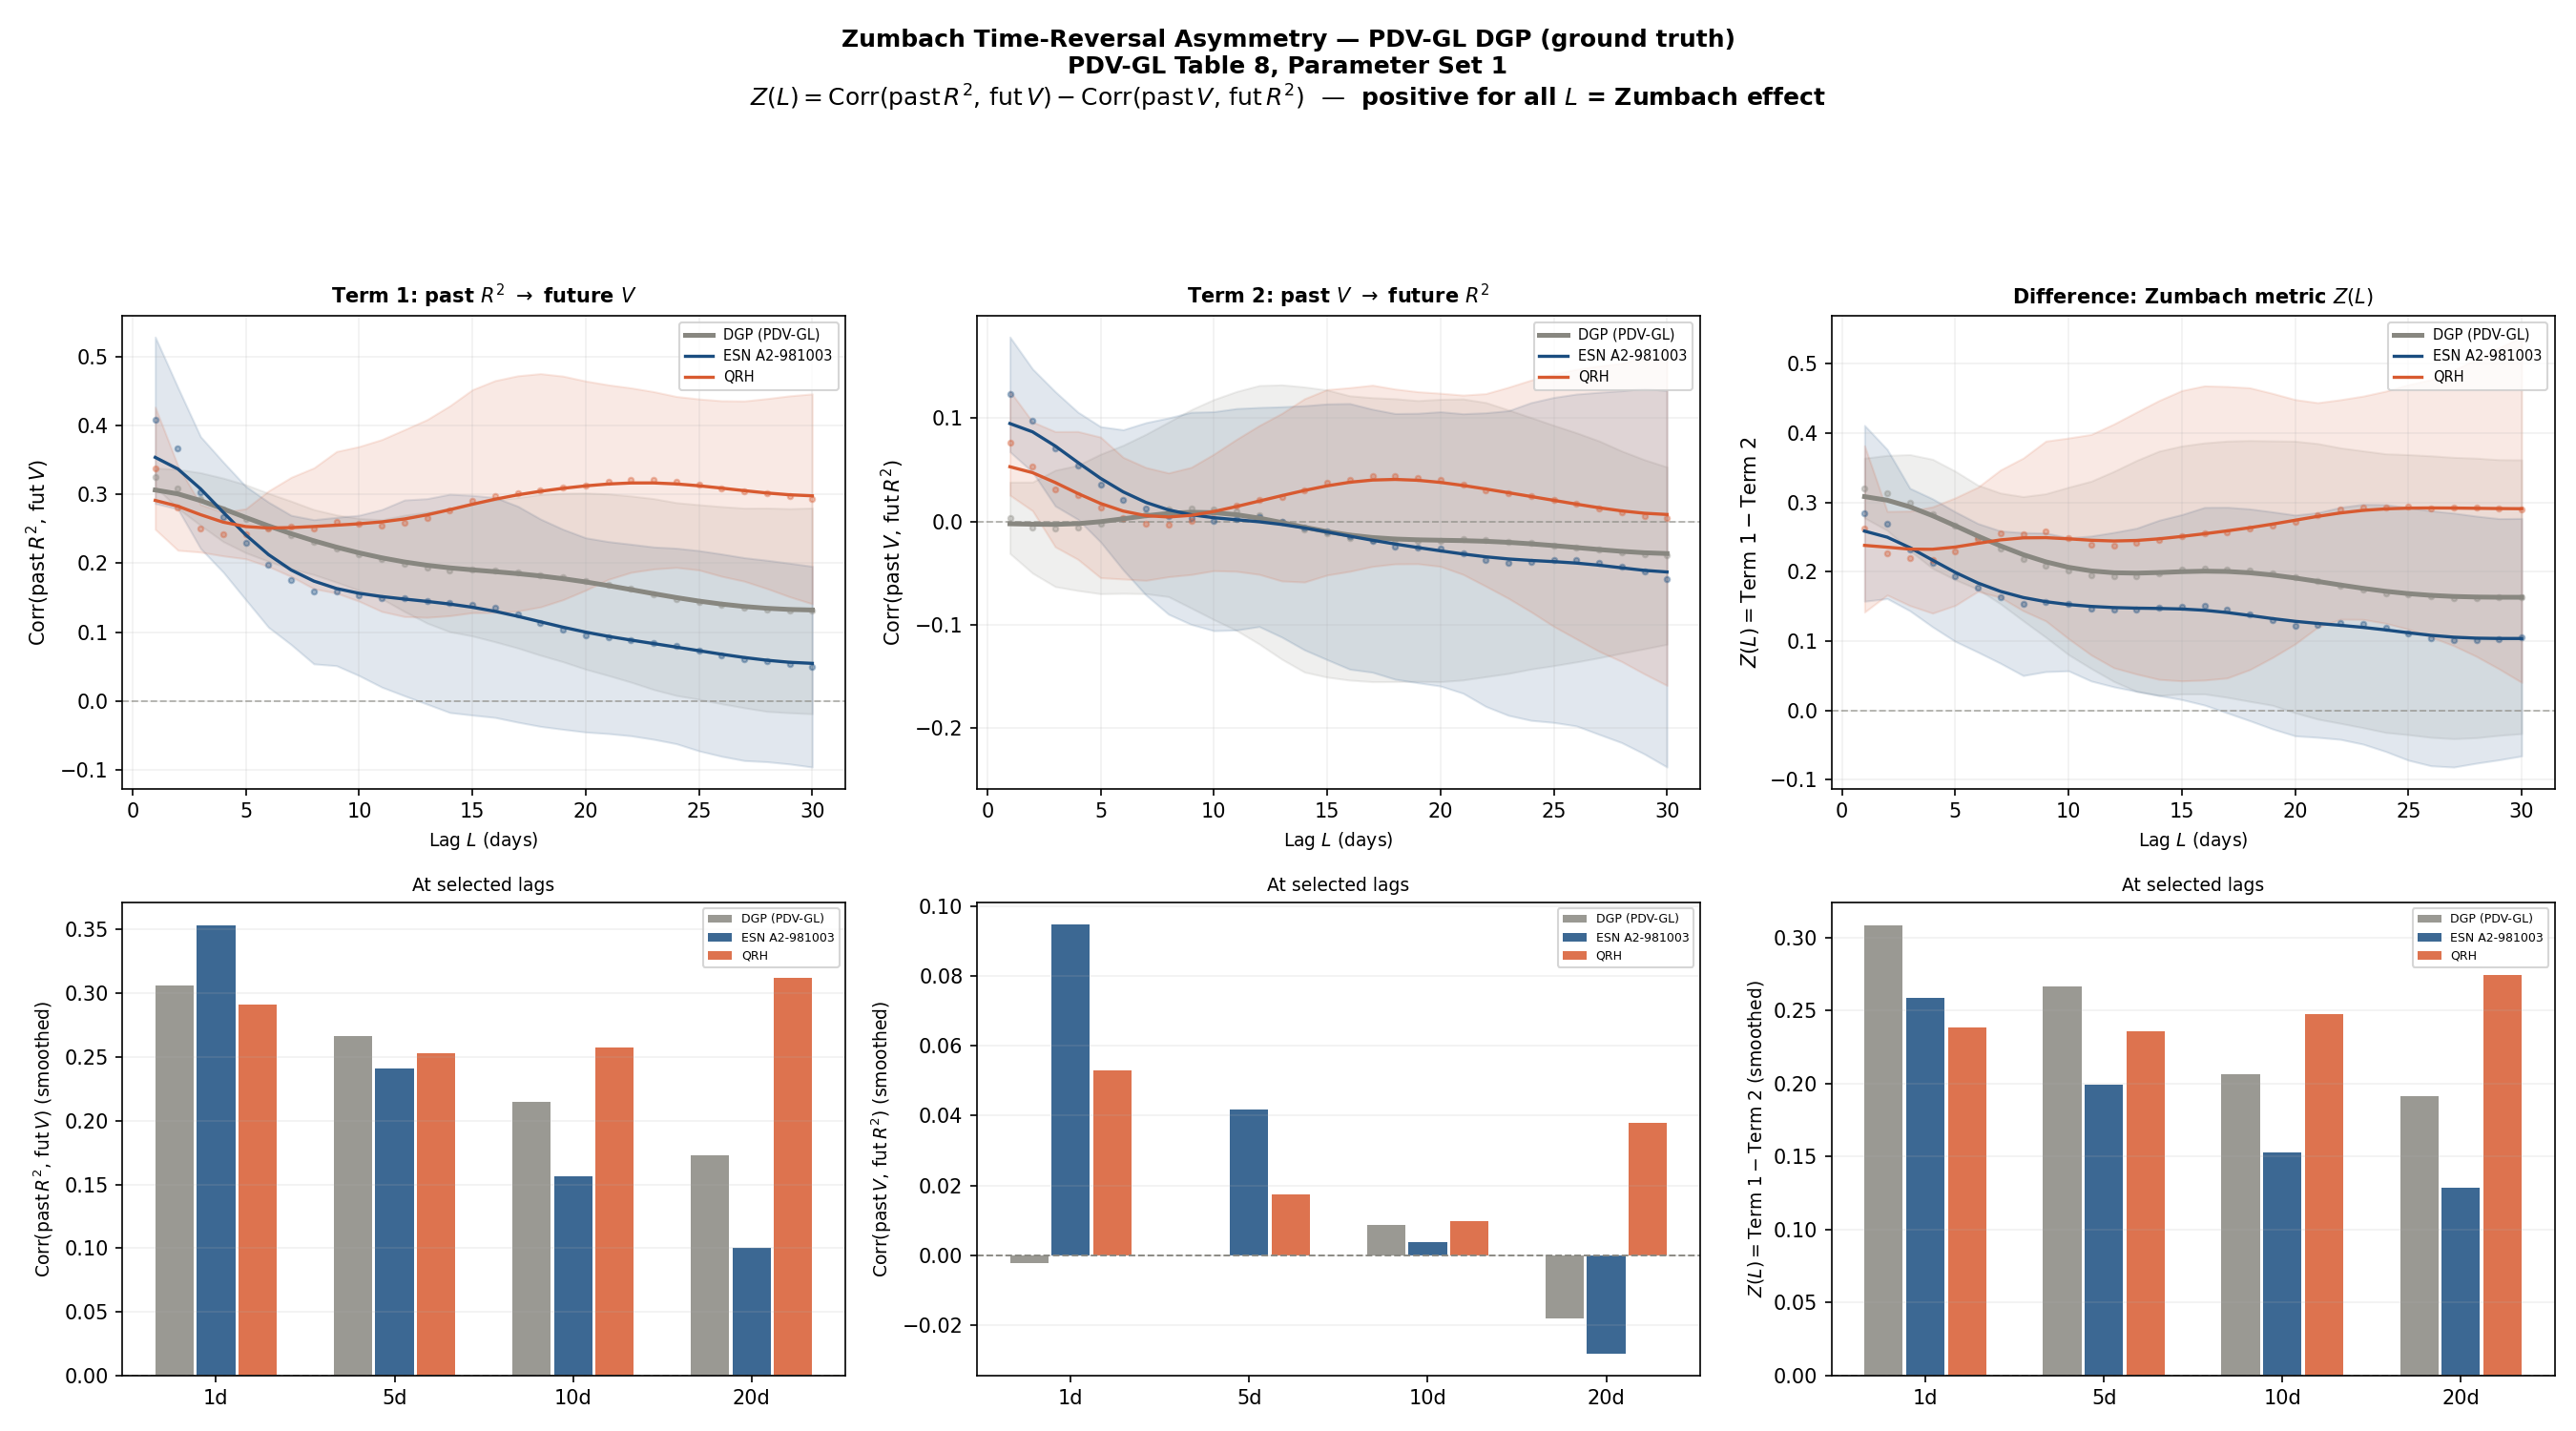
\includegraphics[width=\textwidth]{zumbach_final_out_zumbach_eta0.png}
\caption{Zumbach windowed metric, decomposed into its two terms. Column 1: $\mathrm{Corr}(\mathrm{past}\,R^2,\mathrm{fut}\,V)$ (the genuine, forward Zumbach channel); column 2: $\mathrm{Corr}(\mathrm{past}\,V,\mathrm{fut}\,R^2)$ (the reverse, time-reversed channel); column 3: $Z(L)=$ column 1 $-$ column 2 (the Zumbach metric itself). Top row: curve vs.\ lag (Gaussian-smoothed mean $\pm1$ std band); bottom row: grouped bars at lags 1d, 5d, 10d, 20d. Showing the two terms side by side makes it possible to see whether a model matches the DGP's $Z(L)$ because both terms individually match, or because two mismatched terms happen to cancel to a similar difference.}
\label{fig:zumbachmain}
\end{figure}

\begin{figure}[H]
\centering
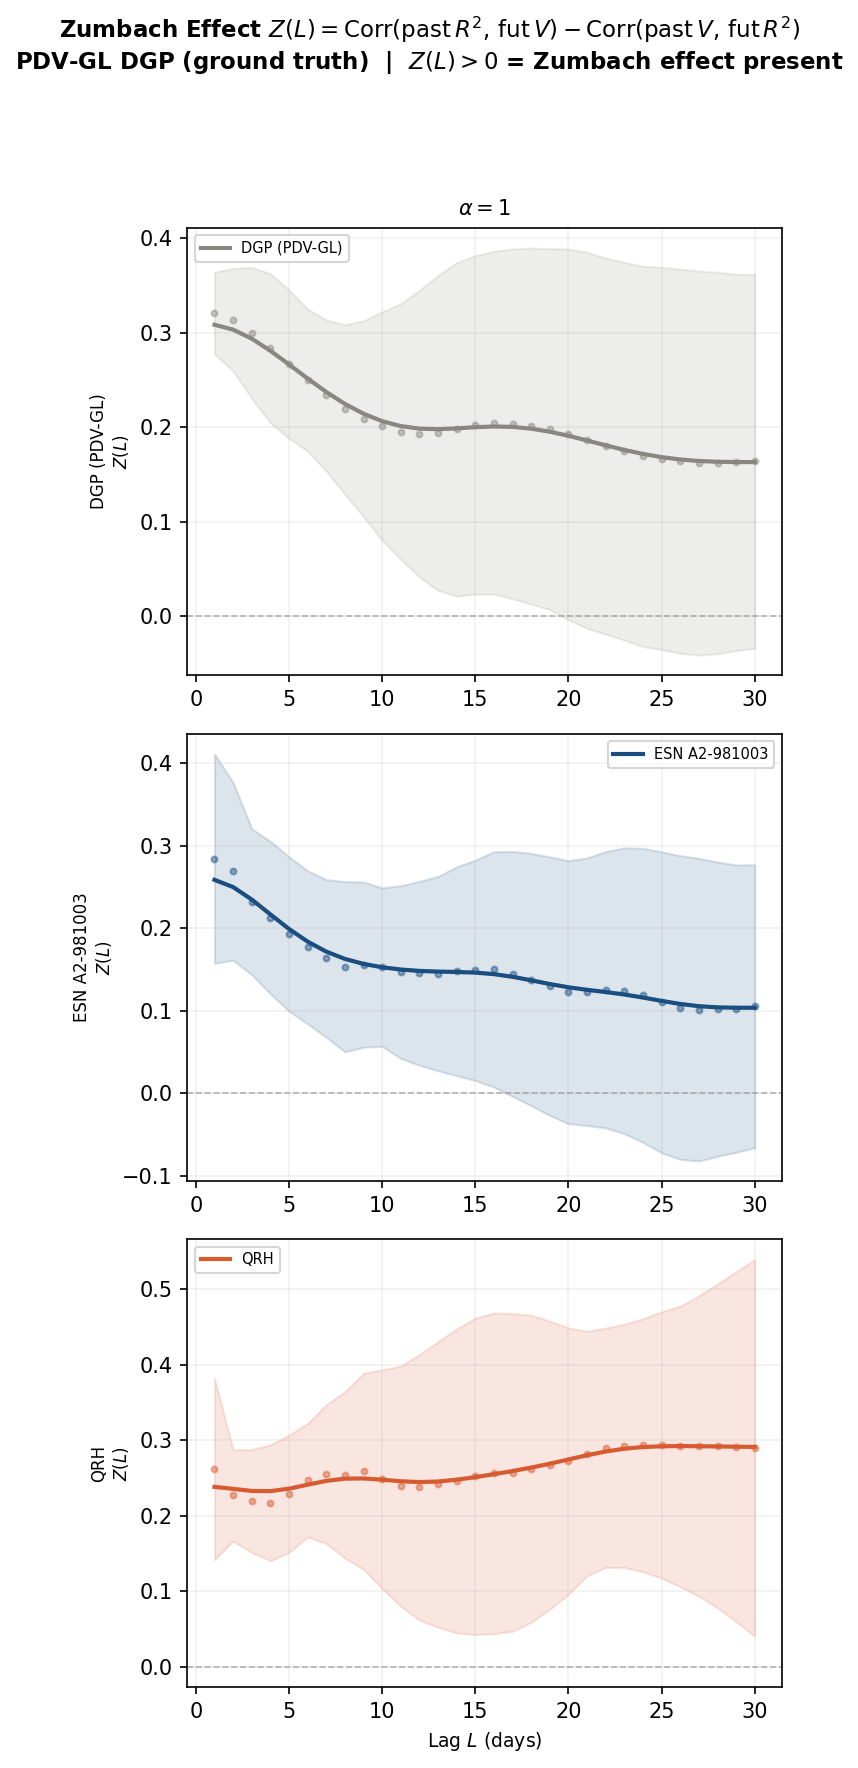
\includegraphics[width=0.55\textwidth]{zumbach_final_out_Z1_eta0.png}
\caption{Windowed $Z(L)$ curves, one row per source (DGP, ESN, QRH), for the single $\alpha_r$ cell tested. Dots are the raw per-lag statistic; the line is Gaussian-smoothed ($\sigma_{\rm sm}=2$ days); the shaded band is $\pm1$ std across paths.}
\label{fig:zumbachZ1}
\end{figure}

\section{Figures}

\textbf{Main figure (Zumbach windowed metric), reproduced above as
Figure~\ref{fig:zumbachmain}, and Figure~\ref{fig:zumbachZ1} (Figure
Z1)} are placed in \S\ref{sec:windowed}, alongside the metric they
illustrate.


\begin{figure}[H]
\centering
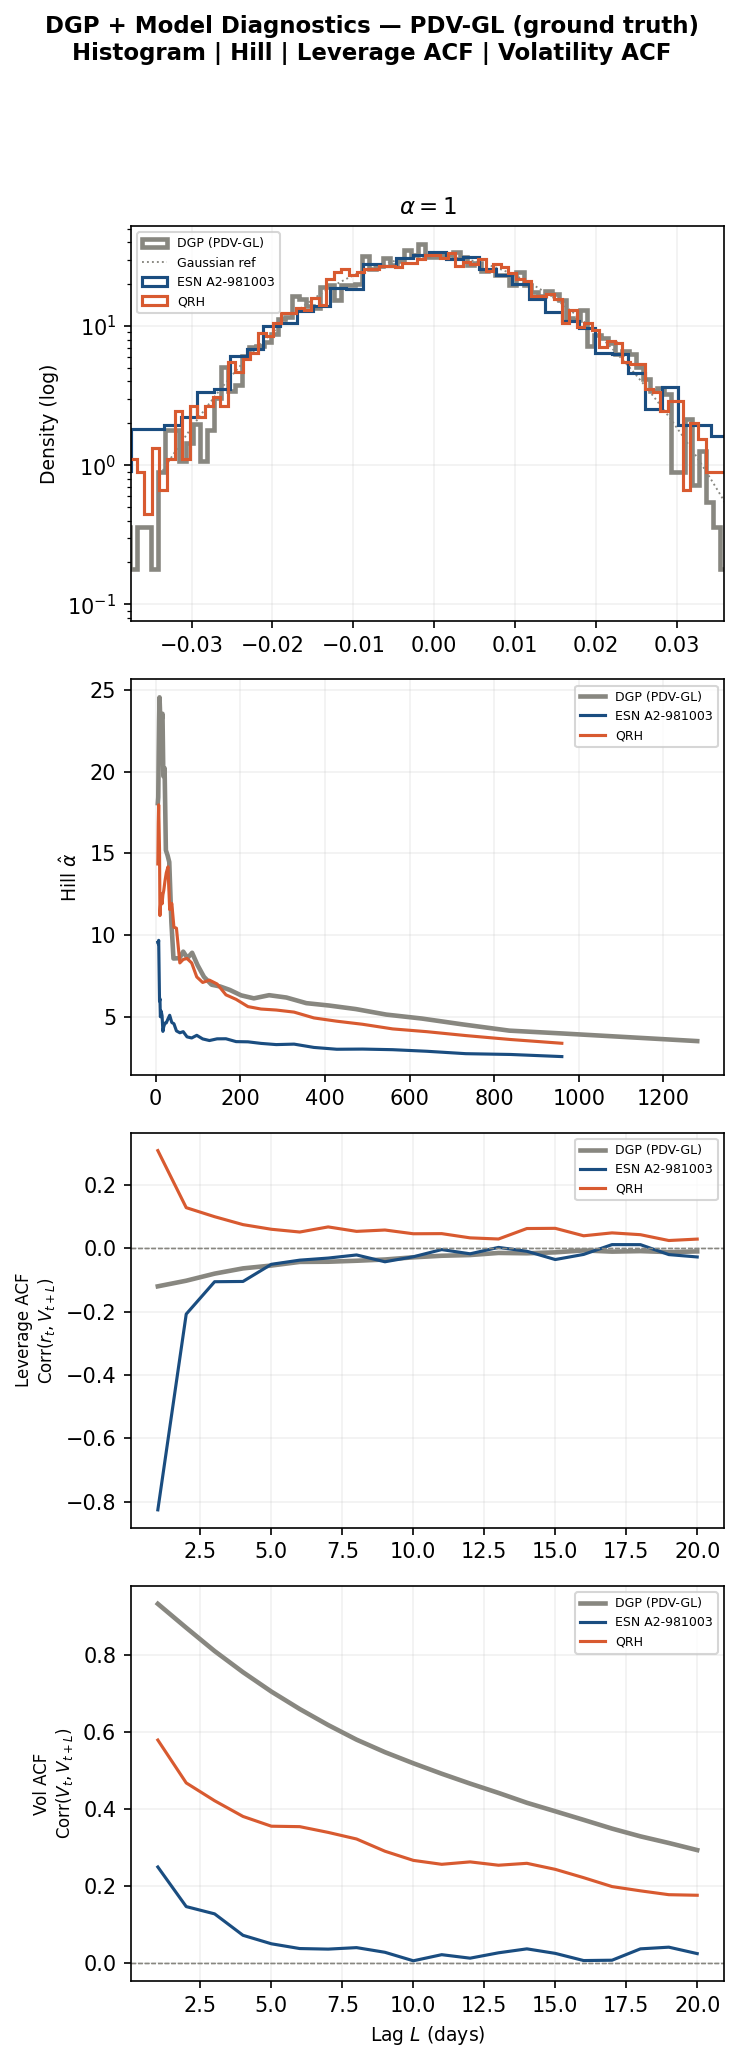
\includegraphics[width=0.5\textwidth]{zumbach_final_out_Z3_eta0.png}
\caption{Return and volatility diagnostics, DGP vs.\ ESN vs.\ QRH: log-density histogram vs.\ Gaussian reference (top); Hill estimator $\hat\alpha$ (second); leverage ACF $\mathrm{Corr}(r_t,V_{t+L})$ (third); volatility ACF $\mathrm{Corr}(V_t,V_{t+L})$ (bottom).}
\label{fig:zumbachZ3}
\end{figure}



\section{Monte Carlo Setup}

\begin{center}\renewcommand{\arraystretch}{1.4}
\begin{tabular}{ll}\toprule Parameter & Value \\\midrule
DGP paths $n_{\rm dgp}$ & 30 \\
Calibration paths $n_{\rm cal}$ & 5 \\
Calibration days $T_{\rm cal}$ & 600 \\
Calibration burn-in & 150 \\
Final paths $n_{\rm sim}$ & 30 \\
Final days $T_{\rm sim}$ & 2500 \\
Final burn-in & 500 \\
$\Delta t$ & 1 (daily) \\
DGP & PDV-GL Table 8, Parameter Set 1 (fixed, no grid) \\
DGP $\beta_0,\beta_1,\beta_2$ & $0.04,\ -0.13,\ 0.65$ \\
DGP $\lambda_{1,0},\lambda_{1,1},\theta_1$ & $55,\ 10,\ 0.25$ \\
DGP $\lambda_{2,0},\lambda_{2,1},\theta_2$ & $20,\ 3,\ 0.5$ \\
Smoothing $\sigma$ & 2 days \\
\bottomrule\end{tabular}\end{center}

\begin{thebibliography}{9}
\bibitem{guyon2023} J.\ Guyon, J.\ Lekeufack.
\textit{Volatility is (mostly) path-dependent}. QF 23(9), 2023.
\bibitem{zumbach2010} G.\ Zumbach.
\textit{Time reversal invariance in finance}. Quantitative Finance
9(5):505--515, 2010.
\end{thebibliography}
\end{document}
